\documentclass[12pt,slidestop]{beamer}
\usepackage[utf8]{inputenc}
\usepackage{german}
\usepackage{graphicx}
\usepackage{tikz}
\beamertemplatenavigationsymbolsempty
\usetheme{Boadilla}
\usecolortheme{whale}
\setbeamertemplate{itemize items}[default]
\setbeamertemplate{enumerate items}[default]
\defbeamertemplate*{footline}{my infolines theme} {
\leavevmode
\hbox{
\begin{beamercolorbox}[wd=.333333\paperwidth,ht=2.25ex,dp=1ex,center]{author in head/foot}
\usebeamerfont{author in head/foot}\insertshortauthor
\end{beamercolorbox}
\begin{beamercolorbox}[wd=.333333\paperwidth,ht=2.25ex,dp=1ex,center]{title in head/foot}
\usebeamerfont{title in head/foot}\insertshorttitle
\end{beamercolorbox}
\begin{beamercolorbox}[wd=.309\paperwidth,ht=2.25ex,dp=1ex,center]{date in head/foot}
\usebeamerfont{date in head/foot}\insertshortdate{}\hspace*{2em}
\insertframenumber{} / \inserttotalframenumber\hspace*{2ex}
\end{beamercolorbox}}
\vskip0pt
}
\newcounter{FrameCounter}
\newcommand{\nextframe}[0]{\stepcounter{FrameCounter}}
\newcommand{\framecount}[1]{\frametitle{\arabic{FrameCounter}. {#1}}}
\newcommand{\fitem}{\vfill\item}
\newcommand{\TikZ}{Ti\textit{k}Z}

\title{FSML++ + Testing}
\author{Carsten Hartenfels \and Benjamin Haßel}
\date{2014-02-26}

\begin{document}
 
\begin{frame}
	\titlepage
\end{frame}

\begin{frame}
	\frametitle{Contents}
	\begin{enumerate}
		\fitem Frameworks
		\fitem Basic Testing	
		\fitem Test Data Generation
		\fitem Extended Testing
		\fitem Running It
		\fitem Questions and Answers
	\end{enumerate}\vfill
\end{frame}

\nextframe
\begin{frame}
	\framecount{Frameworks}\pause
	\begin{itemize}[<+->]
		\fitem Many available...
		\fitem ...but unsuitable to our approach
		\fitem Simple algorithm
	\end{itemize}\vfill
\tikz[remember picture,overlay]
 \node at ([xshift=-2.5cm,yshift=-5cm]current page.north east) 
  {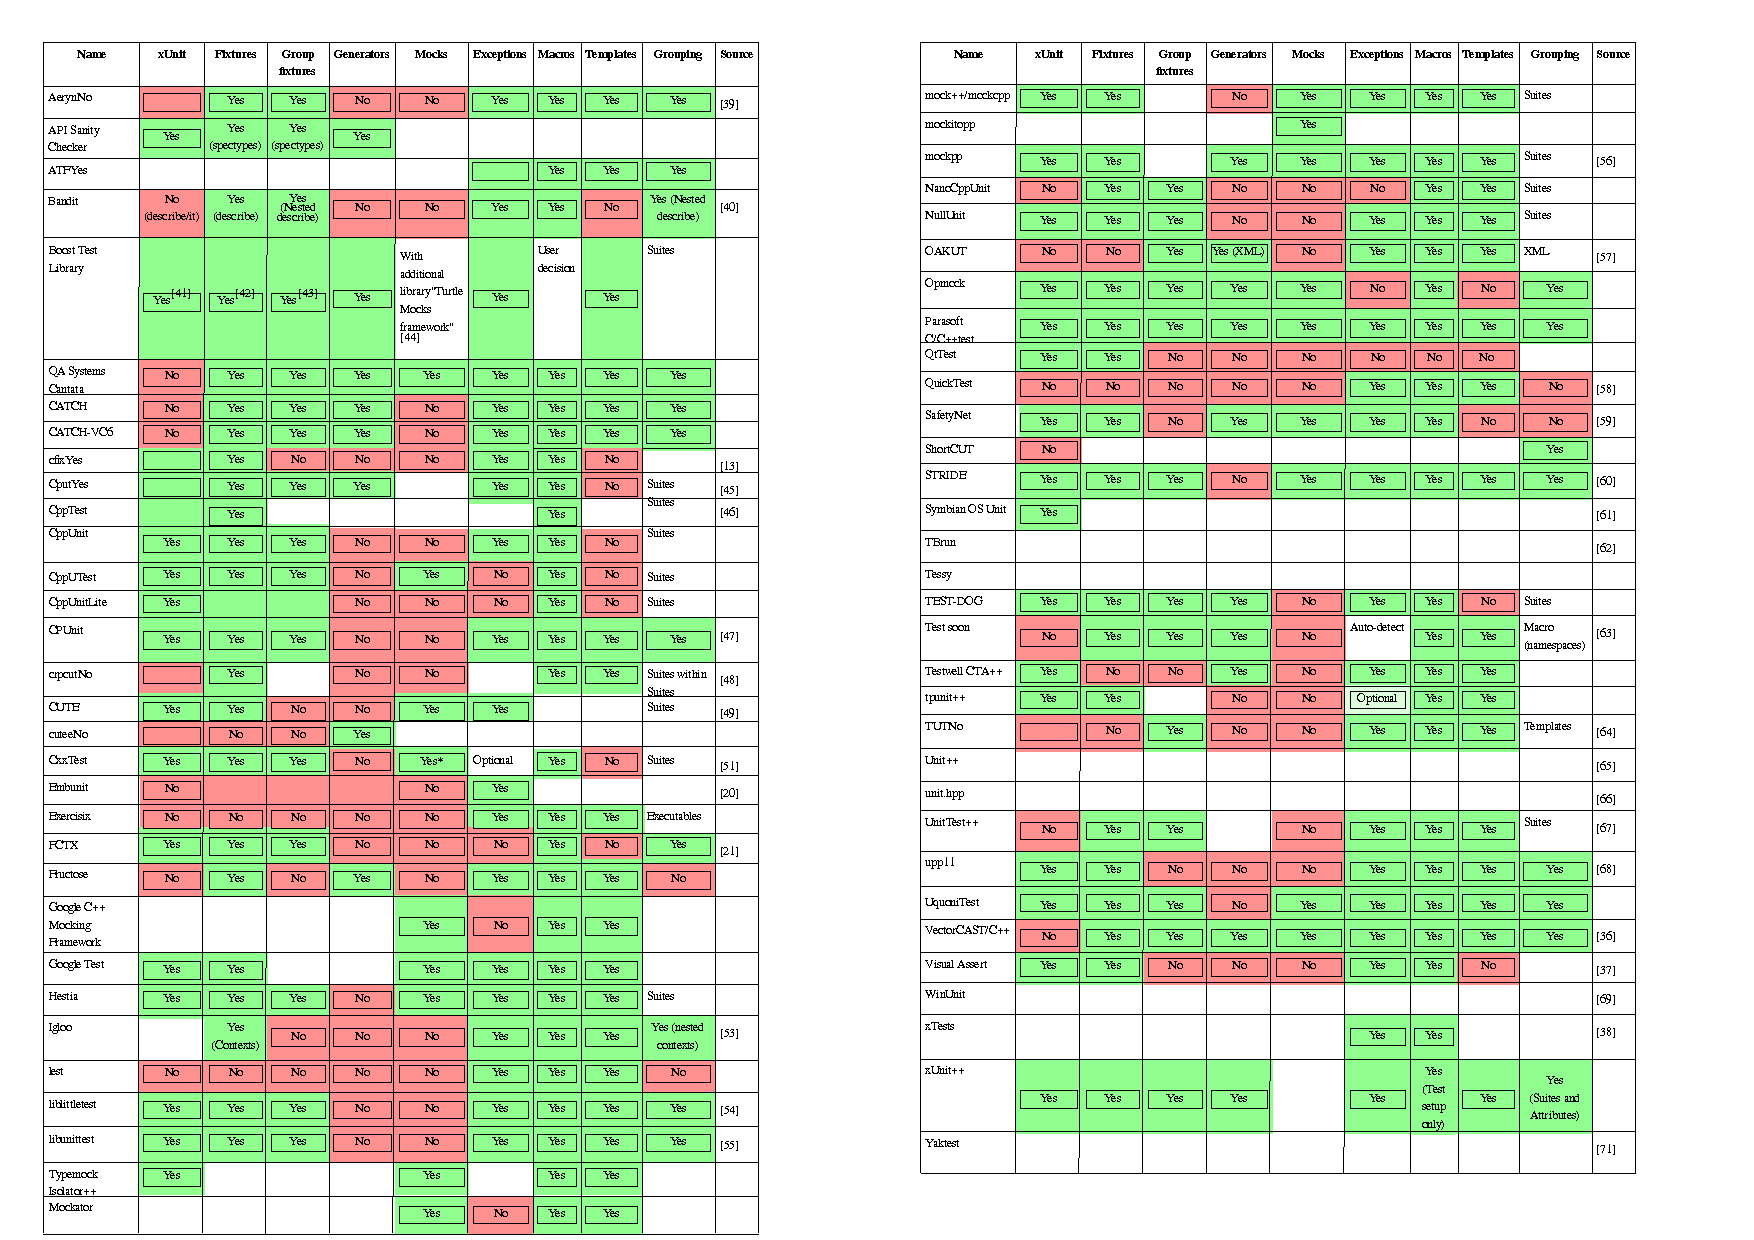
\includegraphics[scale=0.18]{res2/listframeworks_both_1page.pdf}};
\end{frame}

\nextframe
\begin{frame}
	\framecount{Basic Testing}\pause
	\begin{itemize}
		\fitem Identity Testing\pause
		\fitem Testing parser, abstract syntax and flat representation
	\end{itemize}\vfill
	\begin{center}
		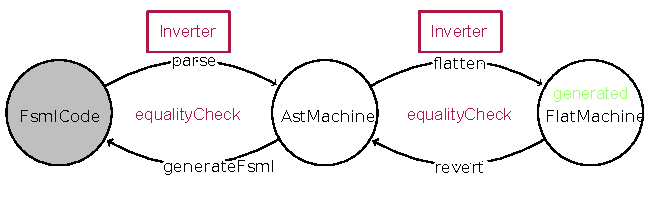
\includegraphics[width=300pt]{res3/leftSideTesting.pdf}		
	\end{center}
\end{frame}

\nextframe
\begin{frame}
	\framecount{Test Data Generation}
	\begin{itemize}
		\fitem Goedelization \tiny(2 states / 25 configurations)
	\end{itemize}	
	\tiny	
	\begin{center}	
	\begin{tabular}{c|lcr}
		\textbf{Goedel Number} &  & \textbf{Transition} &  \\\hline
	 	0&&&\\\hline
		1&s0 $\rightarrow$ s0&&\\\hline
		2&s1 $\rightarrow$ s0&&\\\hline
		3&s0 $\rightarrow$ s1&&\\\hline
		4&s1 $\rightarrow$ s1&&\\\hline
		5&s0 $\rightarrow$ s0&s0 $\rightarrow$ s0&\\\hline
		6&s1 $\rightarrow$ s0&s0 $\rightarrow$ s0&\\\hline
		7&s0 $\rightarrow$ s1&s0 $\rightarrow$ s0&\\\hline
		8&s1 $\rightarrow$ s1&s0 $\rightarrow$ s0&\\\hline
		9&s0 $\rightarrow$ s0&s1 $\rightarrow$ s0&\\\hline
		10&s1 $\rightarrow$ s0&s1 $\rightarrow$ s0&\\\hline
		11&s0 $\rightarrow$ s1&s1 $\rightarrow$ s0&\\\hline
		12&s1 $\rightarrow$ s1&s1 $\rightarrow$ s0&\\\hline
		13&s0 $\rightarrow$ s0&s0 $\rightarrow$ s1&\\\hline
		14&s1 $\rightarrow$ s0&s0 $\rightarrow$ s1&\\\hline
		15&s0 $\rightarrow$ s1&s0 $\rightarrow$ s1&\\\hline
		16&s1 $\rightarrow$ s1&s0 $\rightarrow$ s1&\\\hline
		17&s0 $\rightarrow$ s0&s1 $\rightarrow$ s1&\\\hline
		18&s1 $\rightarrow$ s0&s1 $\rightarrow$ s1&\\\hline
		19&s0 $\rightarrow$ s1&s1 $\rightarrow$ s1&\\\hline
		20&s1 $\rightarrow$ s1&s1 $\rightarrow$ s1&\\\hline
		21&s0 $\rightarrow$ s0&s0 $\rightarrow$ s0&s0 $\rightarrow$ s0\\\hline
		22&s1 $\rightarrow$ s0&s0 $\rightarrow$ s0&s0 $\rightarrow$ s0\\\hline
		23&s0 $\rightarrow$ s1&s0 $\rightarrow$ s0&s0 $\rightarrow$ s0\\\hline
		24&s1 $\rightarrow$ s1&s0 $\rightarrow$ s0&s0 $\rightarrow$ s0\\\hline
		25&s0 $\rightarrow$ s0&s1 $\rightarrow$ s0&s0 $\rightarrow$ s0
 	\end{tabular}
	\end{center}
\end{frame}

\begin{frame}
	\framecount{Test Data Generation}
	\begin{itemize}
		\fitem Algorithm
	\end{itemize}\vfill	
	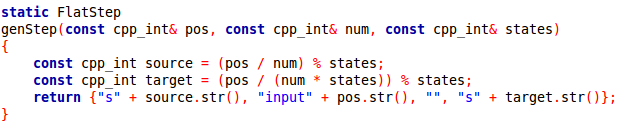
\includegraphics[scale=0.5]{res3/genStep.png}\\ 
	\vfill
	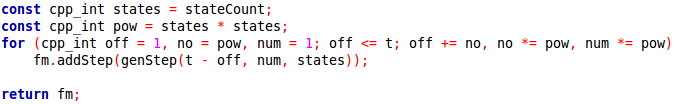
\includegraphics[scale=0.5]{res3/generateFlatMachine.png}
	\vfill
\end{frame}

\nextframe
\begin{frame}
	\framecount{Extended Testing}
	\begin{itemize}
		\fitem Problem: Constraints are not fulfilled\pause
		\fitem Solution: Boost.Graph as oracle
	\end{itemize}\vfill
	\begin{center}
		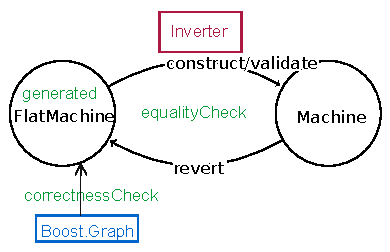
\includegraphics[scale=1]{res3/rightSideTesting.pdf}
	\end{center}
	\vfill
\end{frame}

\nextframe
\begin{frame}
	\framecount{Running It}
	\begin{center}\vspace{70pt}
		{\Huge Example}\\\vspace{54.35pt}
	\end{center}
\end{frame}

\nextframe
\begin{frame}
	\begin{center}\vspace{70pt}
		{\Huge Thank You All For Listening}\\\vspace{54.35pt}
		GitHub: \url{https://github.com/hartenfels/FSMLplusplus/}
	\end{center}
\end{frame}
\end{document}
